\chapter{Literature Review} \label{chap:literature}


\section{Overview}
Drift detection addresses the problem that the statistical properties of data change over time in a way that affects the validity of a machine learning model \citep{Lu2018, Gama2014}. According to \citet{Bayram2022}, when users, environments, or the relationships between labels and features change, model accuracy can decline. \citet{Gama2014} and \citet{Sculley2015} emphasise that drift detection identifies such changes early, so that practitioners can adapt, retrain, or update the model. Figure~\ref{fig:feature-drift} illustrates the idea behind the discriminative detectors studied in this thesis: when the reference and current distributions overlap, a classifier cannot tell their samples apart, and when the distribution shifts, it can.

This chapter is organised by groups of methods rather than by individual papers. After a short history (Section~\ref{sec:lit-history}) and the definitions of drift (Section~\ref{sec:lit-types}), it compares supervised and unsupervised detectors (Section~\ref{sec:lit-classification}), statistical and distance-based detectors including online calibrated ones (Section~\ref{sec:lit-statistical}), classifier-based detectors built on the classifier two-sample test (C2ST) (Section~\ref{sec:lit-c2st}), and other unsupervised families (Section~\ref{sec:lit-other-unsup}). It then reviews three design questions that every window-based detector must answer: how the reference window is maintained (Section~\ref{sec:lit-reference}), how a detection is turned into a statistical decision (Section~\ref{sec:lit-testing}), and whether that decision remains valid when samples are autocorrelated (Section~\ref{sec:lit-autocorr}). The remaining sections cover drift explanation and localisation, evaluation practice, recent detectors designed for other settings, and adaptation strategies, and the chapter ends with a comparison of the method families and the research gap that motivates this thesis.

\begin{figure}[!htpb]
    \centering
    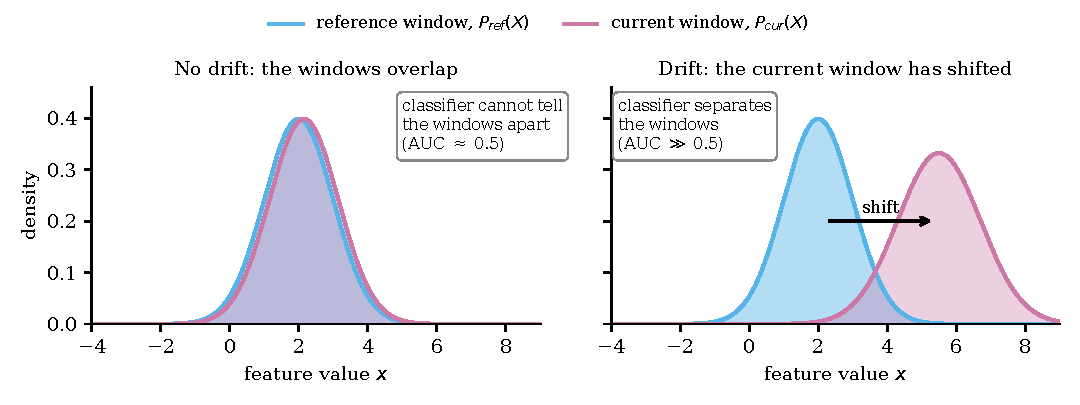
\includegraphics[width=\textwidth]{figures/fig_c2st_concept.pdf}
    \caption[No drift versus drift as a classifier sees it]{No drift versus drift as a classifier sees it. (a) The reference and current windows come from the same distribution, so a classifier cannot tell their samples apart (AUC $\approx$ 0.5). (b) The current window has shifted, so the classifier separates them (AUC $\gg$ 0.5); the arrow marks the shift of the mean.}
    \label{fig:feature-drift}
\end{figure}

\section{Historical Evolution of Drift Detection}
\label{sec:lit-history}
The study of distribution drift has developed from statistical process control to the monitoring of deployed machine learning systems over roughly seven decades. Table~\ref{tab:timeline} summarises the main periods.

\begin{table}[!htbp]
\centering
\caption[Historical evolution of drift detection research]{Historical evolution of drift detection research.}
\label{tab:timeline}
\small
\begin{tabular}{>{\raggedright\arraybackslash}p{3.4cm}>{\raggedright\arraybackslash}p{10.4cm}}
\toprule
Era & Key Developments \\
\midrule
Early Foundations (1950s--1980s) & Statistical process control and sequential analysis laid the groundwork. \citet{Page1954} introduced the cumulative-sum (CUSUM) change-point test, which remains foundational for sequential change detection. Reservoir sampling \citep{Vitter1985} enabled a uniform random sample of a stream of unknown length to be kept in fixed memory. \\
\addlinespace
Identification Era (1996--2004) & The term ``concept drift'', already in use since the 1980s, received an influential early treatment \citep{WidmerKubat1996}. \citet{Gama2004} introduced the Drift Detection Method (DDM), which raises warning and drift alerts when the error rate exceeds its minimum by thresholds derived from the binomial distribution, establishing the supervised error-monitoring paradigm. \\
\addlinespace
Windowing \& Statistical Tests (2007--2016) & \citet{BifetGavalda2007} proposed ADWIN (Adaptive Windowing), which detects change without a fixed window size by testing dynamically adjusted sub-windows. Non-parametric two-sample tests such as the Kolmogorov--Smirnov (KS) test and the Maximum Mean Discrepancy (MMD) became standard for comparing reference and current distributions \citep{Rabanser2019, Gretton2012}, and density-difference tests were adapted to change detection \citep{Bu2017, Bu2018}. \\
\addlinespace
Deep Learning \& High Dimensionality (2017--2023) & Detection moved toward learned representations \citep{Rabanser2019} and two-sample tests on deep-kernel features \citep{Liu2020}. \citet{LopezPazOquab2017} formalised the classifier two-sample test (C2ST), and \citet{Gozuacik2019} applied the same idea to streams in D3. Online detectors with calibrated false detection rates \citep{CobbSequential2022} and sequential two-sample tests by betting \citep{PodkopaevRamdas2023} brought stream-level error control to multivariate tests. \\
\addlinespace
Attribution and Evaluation Era (2024--2026) & Attention moved toward interpretable and statistically rigorous detection: TRIPODD \citep{TRIPODD2024} tests feature interactions; E-C2ST \citep{EC2ST2024} gives anytime-valid C2STs via e-values; HDPD \citep{HDPD2024} decomposes performance gaps into $P(X)$ and $P(y \mid X)$ components. Cloud monitoring services compare the feature attributions of production predictions with a training baseline \citep{TalySato2021, AWSSageMaker2025}. Benchmarks of unsupervised detectors on real streams \citep{Lukats2024} and protocols that inject drift into real data \citep{CerqueiraKDD2026} changed how detectors are evaluated. \\
\bottomrule
\end{tabular}
\end{table}

This progression, from reactive error monitoring to the analysis of feature distributions and attributions with controlled error rates, provides the context for the present work.

\section{Concept Drift: Definitions and Types}
\label{sec:lit-types}
Following \citet{Gama2014}, concept drift between two time points $t_0$ and $t_1$ occurs when the joint distribution of features and labels differs, that is, $P_{t_0}(X, y) \neq P_{t_1}(X, y)$ for some $X$. Because $P(X, y) = P(y \mid X)\,P(X)$, a change can affect the conditional distribution, the feature distribution, or both. \citet{Webb2016} give a formal framework that describes a drift by further quantitative properties, such as its magnitude and duration. Drift can thus be categorised along two dimensions: by the nature of the change (which component of the data-generating process is affected) and by its temporal pattern (how the change unfolds over time) \citep{Lu2018, Gama2014}.

\subsection{Drift by Nature of Change}
Based on which component of the joint distribution $P(X, y)$ changes, the literature \citep{Lu2018, Gama2014, Tsymbal2004} distinguishes the following types.

\textbf{Real Concept Drift:} The conditional distribution $P(y \mid X)$ changes over time while the feature distribution $P(X)$ may or may not change \citep{Lu2018, Zliobaite2010}. The relationship that the model has learned between inputs and outputs is no longer valid. For example, a news reader who has bought a house and starts looking for a holiday destination no longer finds articles on dwelling houses relevant but now finds articles on holiday homes relevant, even though the incoming articles themselves remain similar \citep{Gama2014}. Real drift directly degrades model performance because the learned decision boundaries no longer reflect the true input-output relationship \citep{Lu2018}.

\textbf{Feature Drift (Virtual Drift, Covariate Shift):} The marginal distribution of the input features $P(X)$ changes over time. When the conditional relationship $P(y \mid X)$ remains stable, the change is called virtual drift \citep{Tsymbal2004, Gama2014} or covariate shift \citep{Shimodaira2000}; a change in $P(X)$ can also accompany real drift. The concept itself does not change, but the model may receive inputs outside its training distribution. For example, a fraud detection model trained on transaction patterns from one demographic may receive data from a different user population, even though the definition of fraud remains unchanged. Covariate shift can degrade model performance because the model is exposed to feature regions where it may not generalise well \citep{Shimodaira2000}.

\textbf{Prior Probability Drift (Label Shift):} The marginal distribution of labels $P(y)$ changes over time while $P(X \mid y)$ remains stable \citep{Zliobaite2010}. This occurs when the prevalence of the classes changes, for instance a seasonal increase in a particular disease that alters the class balance in medical diagnosis. This is also called prior probability shift \citep{Lu2018}.

\textbf{Note on Terminology:} The literature uses varied terminology \citep{Lu2018}. The term ``concept drift'' is sometimes used as an umbrella term for any distribution change affecting model performance \citep{Gama2014}, while others distinguish real concept drift, a change in $P(y \mid X)$, from virtual concept drift, a change in the data distribution only \citep{Tsymbal2004}. A detector that sees only the features can observe changes in $P(X)$ but cannot tell whether $P(y \mid X)$ has changed as well. This thesis studies the detection of feature drift, which needs no labels and can warn before the error rate rises; it does not attempt to separate real from virtual drift.

\subsection{Drift by Temporal Pattern}
Based on how drift unfolds over time, the literature \citep{Lu2018, Gama2014, Zliobaite2010, Webb2016} distinguishes four patterns:

\begin{itemize}
    \item \textbf{Abrupt (Sudden) Drift:} A rapid, discrete change where the data distribution shifts from one state to another within a short time period \citep{Gama2014}.

    \item \textbf{Gradual Drift:} A new distribution progressively replacing the old one over an extended duration, with samples from both distributions interleaved during the transition period \citep{Lu2018}.

    \item \textbf{Incremental Drift:} Small but continuous changes accumulating over time, eventually resulting in a significant distributional shift \citep{Zliobaite2010}.

    \item \textbf{Recurring (Seasonal) Drift:} Previously observed distributions reappearing after some time, often periodically due to cyclical patterns, such as seasonal effects in retail or recurring user behaviour \citep{Lu2018, Gama2014}.
\end{itemize}

The patterns place different demands on a detector: abrupt drift requires a rapid response, gradual and incremental drift require sensitivity to changes that are small between neighbouring windows but large over the whole transition, and recurring drift benefits from mechanisms that recognise previously seen distributions \citep{Gama2014}. The second demand is central to this thesis, because it depends on which data the detector compares the current window with (Section~\ref{sec:lit-reference}). Figure~\ref{fig:temporal-patterns} illustrates the four patterns on a synthetic example.

\begin{figure}[!htbp]
    \centering
    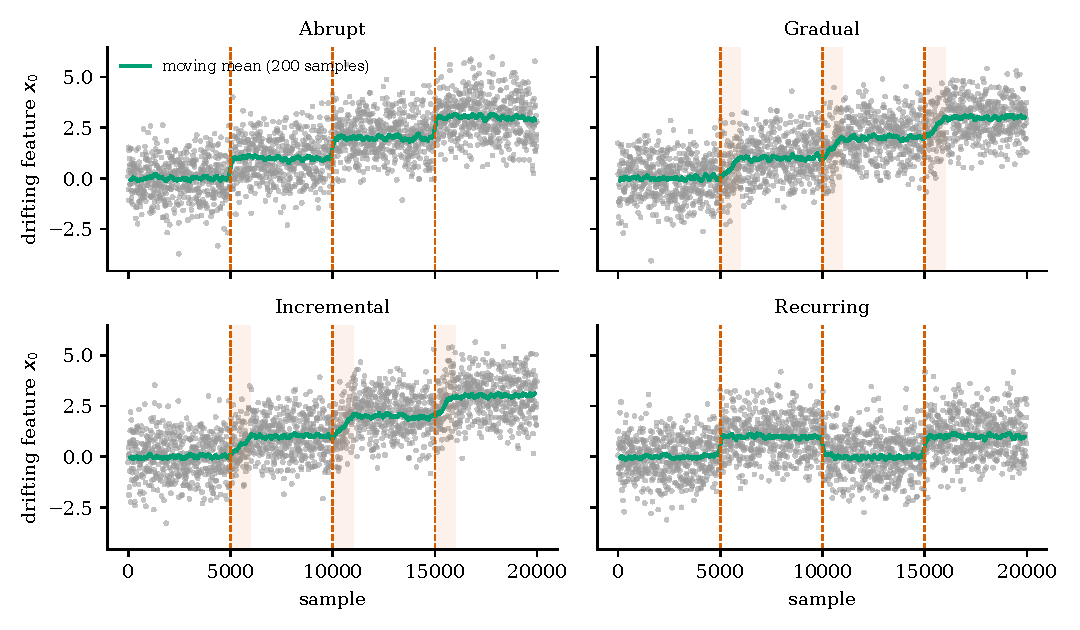
\includegraphics[width=\textwidth]{figures/fig_drift_patterns.pdf}
    \caption[Four temporal drift patterns]{The four drift patterns of the synthetic streams used in this thesis, shown for one drifting feature (seed 0). Grey points are every tenth sample, the green line is a moving mean over 200 samples, dashed lines mark the drift points at 5,000, 10,000 and 15,000, and shaded bands mark the 1,000 samples over which gradual and incremental drift unfold.}
    \label{fig:temporal-patterns}
\end{figure}

\subsection{Summary Taxonomy}
Table~\ref{tab:drift-taxonomy} consolidates the drift classification used throughout this thesis.

\begin{table}[!htbp]
\centering
\caption[Taxonomy of drift types referenced in this thesis]{Taxonomy of drift types referenced in this thesis.}
\label{tab:drift-taxonomy}
\small
\begin{tabular}{>{\raggedright\arraybackslash}p{2.5cm}>{\raggedright\arraybackslash}p{3.4cm}>{\raggedright\arraybackslash}p{7.2cm}}
\toprule
Category & Type & Description \\
\midrule
\multirow[t]{3}{*}{\parbox[t]{2.5cm}{\raggedright By Nature of Change \\ \citep{Lu2018, Gama2014}}}
  & Feature Drift (Covariate Shift) & Change in the input distribution $P(X)$; virtual drift when $P(y \mid X)$ stays the same. \\
  \addlinespace
  & Real Concept Drift & Change in the conditional $P(y \mid X)$, invalidating learned decision boundaries. \\
  \addlinespace
  & Prior Probability Drift & Change in the label distribution $P(y)$ while $P(X \mid y)$ is stable. \\
\midrule
\multirow[t]{4}{*}{\parbox[t]{2.5cm}{\raggedright By Pattern \\ \citep{Gama2014, Zliobaite2010}}}
  & Abrupt (Sudden) & Rapid, discrete shift between two distinct distributions. \\
  \addlinespace
  & Gradual & Old concept progressively replaced by a new one over an extended period. \\
  \addlinespace
  & Incremental & Small, continuous changes accumulating into a significant shift. \\
  \addlinespace
  & Recurring (Seasonal) & Previously observed distributions reappearing, periodically or irregularly. \\
\bottomrule
\end{tabular}
\end{table}

\section{Supervised and Unsupervised Detectors}
\label{sec:lit-classification}
Surveys of the concept drift literature classify drift detection methods along several dimensions \citep{Lu2018, Gama2014, Tsymbal2004, Hinder2024}. According to \citet{Lu2018}, detection algorithms can be grouped by the test statistic they apply (error rate-based, data distribution-based or multiple hypothesis tests). A further distinction, used in this thesis, is based on label availability: whether the method requires ground-truth labels (supervised) or operates without them (unsupervised).

\subsection{Supervised Detectors}
Supervised detectors require ground-truth labels and monitor the error stream of the deployed model \citep{Gama2014, Gama2004}. They assume that a change in error behaviour, such as a higher error rate, errors that occur closer together, or a shift in the mean of a monitored loss, indicates drift \citep{Gama2004, BaenaGarcia2006}. The methods in this group differ mainly in the statistic they track and in the bound they use to decide that a change is significant. DDM compares the error rate and its standard deviation with thresholds derived from the binomial distribution \citep{Gama2004}. EDDM tracks the distance between consecutive errors, which makes it more sensitive to gradual drift \citep{BaenaGarcia2006}. The Page--Hinkley test accumulates the deviations of the monitored signal from its mean \citep{Page1954}, and the Hoeffding drift detection methods HDDM-A and HDDM-W replace distributional assumptions with Hoeffding-type bounds, using moving averages for abrupt change and weighted moving averages for gradual change \citep{FriasBlanco2015}.

Because these methods all watch the model's errors, they share the same strengths and weaknesses. Their alarms are tied directly to model performance, and their thresholds have a clear statistical meaning. However, they need labels, which are often delayed, expensive, or unavailable in production \citep{Lu2018, Sethi2017}. They also react only after drift has already degraded performance, and they cannot detect a change in $P(X)$ that has not yet affected the error rate.

\subsection{Unsupervised Detectors}
Unsupervised detectors do not require ground-truth labels and instead monitor changes in the data distribution, the outputs of a model, or internal representations \citep{Tsymbal2004, Hinder2024}. They can detect distributional shifts before performance degradation becomes observable, which makes them valuable in production environments with label delays \citep{Sethi2017}. Most of them follow the same template: they compare a \emph{reference window} with a \emph{current window} of recent samples and raise an alarm when the two differ by more than a threshold or a test allows. The groups below differ in how they measure the difference (Sections~\ref{sec:lit-statistical} to~\ref{sec:lit-other-unsup}); the choice of reference and decision rule is discussed separately in Sections~\ref{sec:lit-reference} and~\ref{sec:lit-testing}, because these choices are shared across groups.

\section{Statistical and Distance-Based Detectors}
\label{sec:lit-statistical}
Statistical detectors compare the reference and current windows through a hypothesis test or a distance measure \citep{Rabanser2019, Raab2020, BifetGavalda2007}. They can be grouped by whether they work on one feature at a time or on the joint distribution, and by whether they test batches or update a statistic online.

\subsection{Univariate Tests}
ADWIN compares the means of sub-windows of an adaptive window and shrinks the window when they differ, with guarantees on its false positive and false negative rates \citep{BifetGavalda2007}. Kolmogorov--Smirnov Windowing (KSWIN) applies the KS test to one feature at a time over sliding windows \citep{Raab2020}. The Population Stability Index (PSI) compares binned distributions of single features against a rule-of-thumb threshold \citep{Yurdakul2018}. These methods are simple and label-free, but with $d$ features they require $d$ tests, so unless the significance level is corrected, the probability of at least one false alarm grows with $d$ \citep{Rabanser2019}, and changes in the joint distribution that leave every marginal unchanged are missed.

\subsection{Multivariate Kernel and Density-Difference Tests}
Divergence measures such as the Kullback--Leibler divergence, the Jensen--Shannon divergence and the Hellinger distance quantify how far apart two estimated distributions are \citep{Dasu2006, DitzlerPolikar2011}. The MMD compares whole multivariate distributions through kernel mean embeddings and gives a two-sample test whose null distribution can be obtained by permutation or by asymptotic arguments \citep{Gretton2012}. The least-squares density difference (LSDD) estimates the integrated squared difference between the two densities directly, without estimating either density, and has been turned into a change detection test \citep{Bu2018} and an incremental version for streams \citep{Bu2017}. These tests avoid the per-feature multiple-testing problem, but their power depends on the kernel and its bandwidth \citep{Gretton2012}, and on high-dimensional data they are usually applied after a dimensionality reduction \citep{Rabanser2019}. Learned deep kernels address the kernel choice at the cost of training a network \citep{Liu2020}.

\subsection{Online Calibrated Detectors}
Batch tests are designed for one comparison. A stream detector repeats the comparison many times, so even a test that holds its level at every step accumulates false alarms over the stream. \citet{CobbSequential2022} address this for MMD and LSDD statistics that are updated sample by sample: they set time-varying thresholds by simulation so that, without drift, the detector reaches a desired expected run time (ERT), the average number of steps before a false detection, while keeping the false positive rate constant across time steps. They also reduce the cost of the quadratic-time MMD estimator during operation from $O(N^2)$ to $O(N)$ for $N$ reference samples. These detectors are implemented as MMD-Online and LSDD-Online in the Alibi Detect library, whose documentation states that online detectors assume a large, fixed reference set and a short test window that slides over the stream \citep{AlibiDetect}. Their strength is a false alarm rate that is calibrated over the whole stream rather than per test; their requirements are a fixed reference, a choice of ERT and window size, and a kernel or density-difference statistic with the same power limitations as the batch tests.

Table~\ref{tab:method-comparison} compares two widely used univariate methods with the multivariate discriminative approach used in this thesis.

\begin{table}[!htbp]
\centering
\caption[Comparison of drift detection approaches]{Comparison of two univariate drift detection approaches with the discriminative approach.}
\label{tab:method-comparison}
\small
\begin{tabular}{>{\raggedright\arraybackslash}p{2.7cm}>{\raggedright\arraybackslash}p{3.5cm}>{\raggedright\arraybackslash}p{3.5cm}>{\raggedright\arraybackslash}p{3cm}}
\toprule
Method & Approach & Strengths & Limitations \\
\midrule
PSI (Population Stability Index) & Compares binned distributions of single features; by a rule of thumb, PSI~$>$~0.25 indicates significant drift \citep{Yurdakul2018} & Simple, interpretable, common in credit scoring \citep{Yurdakul2018} & Univariate only; requires binning; misses feature correlations \\
\addlinespace
KS Test (Kolmogorov--Smirnov) & Non-parametric test comparing cumulative distributions per feature & No distributional assumptions; exact p-values & Univariate only; multiple testing problem with many features \\
\addlinespace
Discriminative Classification & Trains classifier to distinguish old vs.\ new data; uses AUC as drift signal & Multivariate; captures feature interactions; single unified test & Requires classifier training; a raw AUC has no calibrated threshold; attribution needs an extra step (e.g.\ SHAP)\\
\bottomrule
\end{tabular}
\end{table}

\section{Classifier-Based Detectors and the C2ST}
\label{sec:lit-c2st}
Classifier-based (discriminative) detectors train an auxiliary classifier to tell reference samples from current samples \citep{LopezPazOquab2017, Pan2020}. If the classifier separates the two sets better than chance, the distributions differ. A high AUC ($\gg 0.5$) indicates that the distributions are separable; an AUC near 0.5 suggests that they are not \citep{Pan2020, Qian2021}. No labels of the task are needed, only the window that each sample came from. The methods in this group differ in three respects: the classifier they use, what they read from it, and how they turn that reading into a decision.

\subsection{The Classifier Two-Sample Test}
The classifier two-sample test (C2ST), formalised by \citet{LopezPazOquab2017}, provides the statistical basis of the approach: under the null hypothesis that the two samples come from the same distribution, the held-out accuracy of the classifier follows a binomial distribution centred on 0.5, which gives an approximate p-value and so controls the Type~I error. \citet{LopezPazOquab2017} also note that the classifier's feature importances can show which features separate the two samples. A permutation test over the window labels is a common alternative that also applies to statistics such as the AUC \citep{Good2005}. E-C2ST replaces the p-value with e-values, which gives anytime-valid tests when data arrive in batches \citep{EC2ST2024}, and maximum concept discrepancy uses contrastive learning as an alternative to classifier-based testing for online drift detection \citep{MCD2024}. C2ST and E-C2ST were designed as two-sample tests rather than as stream detectors: they specify the test but not how the reference is maintained along a stream.

\subsection{Domain Classifiers in Practice}
In industry practice the same idea is called adversarial validation or a domain classifier. \citet{Pan2020} used it at Uber for the MaLTA user targeting system, training a classifier to detect a mismatch between training and deployment data and removing the features that drifted most before training the targeting model, and \citet{Qian2021} applied it to dataset shift in credit scoring. Open-source monitoring libraries offer it for batches of data. NannyML's domain classifier trains LightGBM to separate a reference period from each chunk of production data and raises an alert when the cross-validated AUC leaves a fixed range \citep{NannyML}. Alibi Detect's ClassifierDrift trains a classifier, optionally with stratified cross-validation, and applies a KS test to its out-of-fold probabilities, or a binomial test to the binarised predictions, for reference and test instances; its reference can stay fixed or be updated to the last $N$ instances or by reservoir sampling \citep{AlibiDetect}. The same library offers SpotTheDiffDrift, a constrained classifier whose learned test locations show how the features of the new data differ from the reference \citep{AlibiDetect}. These tools compare batches that the user chooses; NannyML decides by an AUC range alone, whereas Alibi Detect attaches a statistical test.

\subsection{Streaming Classifier-Based Detectors}
D3 applies the domain classifier to data streams: it trains a logistic regression classifier to separate a sliding reference window from the newest samples and signals drift when the AUC reaches a fixed threshold of 0.7 \citep{Gozuacik2019}. It is one of the detectors that a recent benchmark of unsupervised detectors recommends, depending on the evaluation metric \citep{Lukats2024}. D3 applies no significance test, so its threshold has no statistical calibration, and it discards the trained classifier after computing the AUC, so it reports that drift occurred but not which features caused it. Margin density methods such as Margin Density Drift Detection (MD3) instead track the proportion of samples that fall close to the decision boundary of a classifier, and they set their threshold heuristically, as $\theta$ standard deviations from a reference estimated by cross-validation \citep{Sethi2017}.

Compared with the statistical tests of Section~\ref{sec:lit-statistical}, the classifier-based group tests all features jointly with one model and can capture non-linear changes and changes in feature interactions that marginal tests miss \citep{LopezPazOquab2017}, and a tree ensemble needs no kernel choice. Its costs are that a classifier must be trained at every check, that the results depend on the classifier and its hyperparameters, and that a raw AUC has no statistical meaning unless a test is added. Within the group, the batch tests (C2ST, E-C2ST, ClassifierDrift) supply the test but not the stream design, and the streaming detector D3 supplies the stream design but not the test.

\section{Other Unsupervised Detector Families}
\label{sec:lit-other-unsup}
Two further groups of unsupervised detectors work either on learned representations or model outputs, or on clusters and densities of the raw features; both are less suited to the tabular streams studied here.

\subsection{Representation-Based and Output-Based Detectors}
Representation-based methods monitor learned representations rather than raw features \citep{Rabanser2019}, or learn a feature representation for the two-sample test itself \citep{Liu2020}. They apply two-sample tests such as MMD or per-dimension KS tests to low-dimensional representations, such as autoencoder latents or the softmax outputs of a trained classifier \citep{Rabanser2019}, or they borrow ideas from domain adaptation, such as matching the distributions of learned multi-layer features with MMD \citep{Long2016}. These methods suit high-dimensional data such as images, where simple kernels on raw inputs have little power \citep{Liu2020}, but they require a representation model and are less relevant for the tabular streams studied here.

Output-based methods monitor the outputs of the deployed model without checking whether they are correct \citep{Sethi2017, Rabanser2019}. They track the distribution of predicted classes or scores \citep{Rabanser2019}, or the entropy and confidence of the predictions, assuming that rising uncertainty indicates out-of-distribution inputs \citep{Hendrycks2017}. Their weakness is calibration: modern models, deep networks in particular, are often poorly calibrated, and under distribution shift their confidence may not change in step with their errors \citep{Guo2017, Ovadia2019}. They also need a deployed model, so they monitor the change as seen through that model rather than the change in $P(X)$ itself.

\subsection{Clustering, Density and Signal-Reduction Detectors}
\citet{Lukats2024} reviewed ten fully unsupervised drift detectors and evaluated seven of them on eleven real-world data streams; the other three were too slow or depended too much on chance. They found that the number of samples observed was one of the most influential hyperparameters. Apart from D3, the detectors they studied fall into three groups.

Clustering-based detectors summarise each window with clusters and test whether the clusters change. The Clustered Statistical Test Drift Detection Method (CSDDM) reduces dimensionality with principal component analysis (PCA), clusters the data with K-Means, and applies statistical tests to the clusters \citep{CSDDM2021}, while UCDD assigns pseudo-labels from cluster membership and monitors shifts of the cluster boundary \citep{UCDD2020}. Many CSDDM configurations achieved a higher lift-per-drift, a metric of how much classifier accuracy improves per detected drift, than other detectors at a similar number of detections on some streams, although its best values were lower than those of D3 and SPLL \citep{Lukats2024}.

Density-based detectors model the reference distribution and flag new data that fit the model poorly. The Semi-Parametric Log-Likelihood (SPLL) detector fits a semi-parametric density model and monitors the log-likelihood of new observations \citep{SPLL2013}, NN-DVI tracks changes in nearest-neighbour density \citep{NNDVI2018}, the One-Class Drift Detector (OCDD) fits a one-class support vector machine (SVM) to the reference data and counts the samples that fall outside its boundary \citep{OCDD2021}, and the Bayesian Nonparametric Detection Method (BNDM) compares windows with a Bayesian non-parametric P\'{o}lya tree test \citep{BNDM2020}. These detectors respond well to sudden changes in density, but they are sensitive to the size of the reference sample: BNDM signalled drift periodically when it observed few samples, and many OCDD configurations showed the same periodic behaviour \citep{Lukats2024}.

A last group reduces the stream to a simpler signal. The Image-Based Drift Detector (IBDD) converts windows of numerical data into images and compares the images \citep{IBDD2021}, and UDetect \citep{Bashir2017} applies Shewhart control charts to the average distance of the samples in each window to their centre, computed separately for each predicted activity class. IBDD achieved the best classifier accuracy on five of the eleven streams because it can signal drift again immediately after a reset, but it was among the worst detectors on mean time ratio, and 45\% of the UDetect configurations detected no drift at all \citep{Lukats2024}. Across all groups, the benchmarked detectors report whether drift occurred but not where it occurred \citep{Lukats2024}.

\section{Reference Window Strategies}
\label{sec:lit-reference}
Every window-based detector must decide which past data the current window is compared with. Three strategies appear in the literature, and they are shared across the families above.

A \emph{fixed} reference is a sample taken once, for example the training data or a chosen reference period, and kept until the detector is reset. NannyML compares production chunks with a reference period \citep{NannyML}, and the online detectors of \citet{CobbSequential2022} assume a large, fixed reference set \citep{AlibiDetect}. A fixed reference accumulates the whole change since it was taken, so slow drift eventually becomes large relative to it, but it can become stale and must be replaced after an alarm.

A \emph{sliding} reference holds the samples just before the current window and moves with the stream. D3 \citep{Gozuacik2019} and KSWIN \citep{Raab2020} use this design, and ADWIN adapts the window length instead of fixing it \citep{BifetGavalda2007}. A sliding reference stays close to the current data, which keeps false alarms low when the stream changes harmlessly, but under gradual or incremental drift the two adjacent windows differ only by the change that occurred between them. A slow drift can therefore stay below the threshold at every check although the total change is large, which is the difficulty noted for these patterns in Section~\ref{sec:lit-types}.

A \emph{reservoir} reference keeps a uniform random sample of all data seen since the last reset. Reservoir sampling (Algorithm R) maintains such a sample of fixed size from a stream of unknown length by replacing a stored item with decreasing probability \citep{Vitter1985}. It sits between the two other strategies: like a fixed reference, it represents the whole period since the last alarm, and like a sliding reference, it is updated as the stream advances. Alibi Detect already offers reservoir sampling as an option for updating the reference of its batch detectors, including ClassifierDrift \citep{AlibiDetect}. To our knowledge, however, its effect on the detection of slow drift has not been isolated from the other design choices of a detector, such as the classifier, the window sizes and the decision rule.

\section{Permutation and Sequential Testing}
\label{sec:lit-testing}
A detector needs a rule that turns a statistic, such as an AUC or an MMD estimate, into an alarm. Fixed thresholds, as in D3 and NannyML, are simple but have no error guarantee. The tests reviewed here differ in what their error guarantee covers: one test, one test with a resampling budget, or the whole stream.

\subsection{Permutation Tests and Sequential Monte Carlo}
A permutation test compares the observed statistic with its values after the window labels are randomly reassigned, and it is exact when the samples are exchangeable under the null hypothesis \citep{Good2005}. For a C2ST with $B$ permutations, the classifier is retrained $B$ times for each test, which is costly in a stream. Sequential Monte Carlo tests reduce this cost by stopping the resampling once the decision is clear: \citet{BesagClifford1991} give an exact sequential p-value that stops after a fixed number of exceedances, and \citet{Gandy2009} gives a procedure whose probability of reaching a different decision from the full Monte Carlo test is uniformly bounded. These methods control the error of each single test.

\subsection{Sequential Tests over the Stream}
A detector that runs a level-$\alpha$ test at every check still accumulates false alarms over a long stream, because the per-test error applies to every check. Two lines of work control the error over the whole stream instead. The online calibrated detectors of \citet{CobbSequential2022} set their thresholds so that the expected run time without drift reaches a chosen value (Section~\ref{sec:lit-statistical}). Testing by betting builds a test statistic that grows like the wealth of a gambler who bets against the null hypothesis; \citet{PodkopaevRamdas2023} use a sequentially updated classifier as the betting strategy, so that a classifier that keeps predicting which sample an instance came from counts as evidence against the null. Their test controls the Type~I error at any stopping time, and the authors report that it remains valid when the data distribution changes over time. E-C2ST follows a related idea with e-values for batches \citep{EC2ST2024}. Compared with per-test methods, these approaches give a stream-level guarantee, but they treat the data as a sequence of new observations to be tested against one null, rather than comparing a moving current window with a reference that is replaced after each alarm.

\section{Autocorrelation and Exchangeability}
\label{sec:lit-autocorr}
The guarantees above rest on assumptions about the data. A permutation test is valid when the samples are exchangeable under the null hypothesis, that is, when their joint distribution does not change if the samples are reordered \citep{Good2005}. Samples from a stream are often autocorrelated: neighbouring samples are more alike than distant ones, even when the stream is stationary. A window of consecutive samples then varies more than a random sample of the same size, and shuffling the window labels removes this dependence, so the permutation null is too narrow and the test rejects too often. \citet{Chwialkowski2014} show this failure for kernel tests on random processes, where the naive permutation-based bootstrap does not hold its level, and propose a wild bootstrap that does. The same issue applies to a C2ST on a stream, because the reference and current windows are blocks of dependent samples. For a feature drift detector, a rejection on a stationary but autocorrelated stream is a false alarm. To our knowledge, none of the stream detectors reviewed above adapts its null distribution to autocorrelation; among the sequential tests, \citet{PodkopaevRamdas2023} state that their betting tests remain valid when the data distribution changes over time.

\section{Drift Explanation and Localisation}
\label{sec:lit-explanation}

\subsection{Drift Localisation}
Drift localisation asks where a drift occurs \citep{HinderLocalization2024}. The question can be posed for regions of the data space, that is, which samples are affected, or for features, that is, which input dimensions are affected. \citet{HinderLocalization2024} formalise localisation as finding the smallest region of the data space whose removal leaves no drift, and they survey the methods that address it. Most of these methods are built on local drift detection. Binning methods such as kdq-trees partition the data space and compare the samples in each cell \citep{Dasu2006}. Neighbourhood methods compare the local density around each sample, as in the local drift degree of \citet{Liu2017LDD}. Model-based methods train a probabilistic classifier to separate time periods and read the affected regions from its predictions \citep{HinderLocalization2024}.

Feature-level localisation has developed alongside region-level localisation. \citet{Kulinski2020} framed the question of which features have shifted as a set of conditional distribution tests, one per feature, based on the score function of a density model. \citet{HinderFeature2024} gave formal definitions of feature-wise drift that allow detector-agnostic selection of drifting features. TRIPODD \citep{TRIPODD2024} tests feature interactions with power guarantees, but it needs ground-truth labels and a trained model, and because it considers all feature subsets it must sample feature permutations to keep the cost manageable. These methods differ in what they require: a density model \citep{Kulinski2020}, ground-truth labels and a trained model \citep{TRIPODD2024}, or batch access to the data \citep{HinderFeature2024}.

\subsection{Feature Attribution for Drift}
Feature attribution methods explain the output of a model in terms of its input features. SHAP (SHapley Additive exPlanations) assigns each feature its Shapley value \citep{Shapley1953} in a cooperative game whose players are the features \citep{Lundberg2017}, and TreeSHAP computes these values exactly and in polynomial time for tree ensembles \citep{LundbergInteraction2020}. Attribution has been connected to drift in three ways.

The first way explains a domain classifier. \citet{Maggio2021} trained a classifier to separate old data from new data and ranked the features by the mean absolute SHAP value of the classifier's output; in that study, the SHAP ranking identified the corrupted features more reliably than the classifier's impurity-based feature importance. This is the same classifier that a classifier-based detector already trains, so the ranking adds feature-level localisation at little extra cost. Its limitations come from SHAP itself: the attributions describe the classifier rather than the data-generating process, and model-based drift explanations of this kind are exploratory rather than causal \citep{CausalDrift2025}.

The second way monitors the attributions of the deployed model. \citet{LundbergInteraction2020} monitored the SHAP values of a deployed model's loss over time, which requires labels, to find problems in its data pipeline and feature drift. \citet{Mougan2025} defined explanation shift as a change in the distribution of a model's explanations between training data and new data, and showed that it can reveal shifts that change model behaviour, including changes in feature interactions that per-feature tests miss. Google Vertex AI and Amazon SageMaker Clarify compare the feature attributions of production predictions with a baseline computed during training \citep{TalySato2021, AWSSageMaker2025}.

The third way attributes changes in model performance, rather than changes in the data distribution. \citet{Zhang2023Attribution} treated the distributions that make up the data-generating process as players in a cooperative game and attributed a model's performance change to them with Shapley values. HDPD decomposes a performance gap into covariate and conditional components with per-feature attributions \citep{HDPD2024}, DBShap separates virtual and real drift with Shapley values defined over distributions \citep{DBShap2024}, and XPE combines optimal transport with Shapley values to explain how feature shifts affect performance \citep{XPE2024}. HDPD and DBShap require labels on the new data, and XPE requires a trained model and labelled source data.

Across the three ways, the methods that need neither labels nor a deployed model are those that explain a domain classifier. A systematic review of 82 studies found that work on explaining drift lacks benchmark datasets and standardised quantitative metrics, and that 94\% of the studies assess their explanations only qualitatively or visually \citep{XAIDriftSurvey2025}. SHAP ranking of the features that separate two windows has been used before \citep{Maggio2021}, so this thesis does not claim it as a method; what is less established is a quantitative check, against known drifting features, of the ranking that a streaming classifier-based detector produces at the moment it raises an alarm.

\section{Benchmarks and Evaluation Practice}
\label{sec:lit-evaluation}
How a detector is evaluated affects which detector appears best. \citet{Lukats2024} evaluated fully unsupervised detectors on real-world streams whose drift points are unknown, and therefore scored them indirectly, by the accuracy of a classifier that is retrained at each alarm and by measures such as the mean time ratio and lift-per-drift. Indirect scores avoid artificial data, but without known drift points they cannot separate correct detections from false alarms. \citet{CerqueiraKDD2026} propose a framework that injects controlled drifts into real datasets through Monte Carlo trials, so that detections can be scored against known drift points while the data keep their real-world structure, and they recommend tuning detector hyperparameters with a leave-one-dataset-out protocol so that settings are not tuned on the evaluation data. They criticise evaluations that rely only on synthetic generators, use incompatible metrics, or tune hyperparameters without reporting it. Real streams with documented drift points, such as the INSECTS streams \citep{Souza2020}, complement both approaches. The evaluation in this thesis follows these recommendations by combining synthetic, injected and annotated real streams, fixed settings shared by all detectors, and statistics computed over streams (Chapter~\ref{chap:methodology}).

\section{Recent Detectors for Other Settings}
\label{sec:lit-recent}
Several detectors published in 2024--2026 address settings that differ from the one studied here, and they are therefore not included in the experiments. PUDD derives a prediction uncertainty index from a deployed classifier and monitors it instead of the error rate \citep{PUDD2025}; like the output-based methods above, it needs a deployed model. DriftLens detects and explains drift in the embeddings of deep learning models for text, image and audio data \citep{DriftLens2024}, a different data type from the tabular streams used here. The Gaussian Split Detector models the data with Gaussian mixtures to track changes in the decision boundary and aims to detect real drift while ignoring virtual drift \citep{GaussianSplit2024}; it answers a different question from a feature drift detector, which treats any change in $P(X)$ as drift. \citet{Komorniczak2026} detects drift in tabular streams from the reconstruction error of autoencoders and recognises samples of new classes, evaluated on synthetic streams; no code for it had been released when the experiments of this thesis were run.

Other recent work addresses label efficiency, explanation quality and robustness. Semi-supervised and student--teacher methods reduce or remove the need for labels \citep{CDSeer2024, STUDD2022}, and autoregressive error monitoring adds confidence intervals to supervised detection \citep{ADDM2022}. SGShift characterises concept shift with generalised additive models and controls the false discovery rate with knockoffs \citep{SGShift2025}, and \citet{CausalDrift2025} argue that drift explanations need causal rather than correlational attribution to guide remediation. \citet{AdvAttackDrift2024} showed that adversarially constructed data streams can evade common drift detectors, including discriminative ones. Hybrid and ensemble approaches combine several base detectors or signals, although simple detector ensembles have not been shown to perform better than single drift detectors \citep{Krawczyk2017}, and they inherit the label or context requirements of their components.

\section{Drift Mitigation and Adaptation Strategies}
\label{sec:mitigation}
Detecting drift is only the first step; production systems must also respond to it. Drawing on \citet{Lu2018}, \citet{Gama2014} and \citet{Krawczyk2017}, we group mitigation strategies into five categories. \emph{Periodic retraining} retrains the model on the latest data at fixed intervals or when a drift alert arrives; it is simple to operate, but fixed schedules may retrain unnecessarily or react too slowly \citep{Gama2014}. \emph{Weighted retraining} combines old and new data but gives recent examples higher weights, which keeps long-term knowledge while favouring current patterns \citep{Krawczyk2017}. \emph{Ensemble methods} keep several models, for example one per data regime, combine their predictions, and replace poorly performing members after a drift \citep{Krawczyk2017}. \emph{Online or incremental learning} updates the model with each new sample or mini-batch and so adapts naturally to gradual and incremental drift \citep{Gama2014, Ditzler2015}. \emph{Human-in-the-loop} adaptation sends uncertain or drifted samples to experts for labelling, often within a labelling budget \citep{Lu2018}, which matters where errors are costly and labels expensive.

A feature drift detector supplies the trigger for the first, second and fifth strategies, and its feature ranking can guide which inputs to inspect before retraining.

\section{Comparison of Method Families}
\label{sec:lit-comparison}
Table~\ref{tab:family-comparison} summarises the method families reviewed in this chapter along five properties: whether they test the joint feature distribution, whether they need labels or a deployed model, whether their decision comes from a statistical test, which reference they compare with, and whether they report which features drifted.

\begin{table}[!htbp]
\centering
\caption[Comparison of drift detection method families]{Comparison of drift detection method families. ``Model'' means a deployed model trained on labelled data is needed; ``per test'' and ``stream'' state what the error guarantee covers.}
\label{tab:family-comparison}
\footnotesize
\setlength{\tabcolsep}{3pt}
\begin{tabular}{>{\raggedright\arraybackslash}p{2.6cm}>{\raggedright\arraybackslash}p{2.6cm}>{\raggedright\arraybackslash}p{1.3cm}>{\raggedright\arraybackslash}p{1.3cm}>{\raggedright\arraybackslash}p{2.0cm}>{\raggedright\arraybackslash}p{1.6cm}>{\raggedright\arraybackslash}p{1.6cm}}
\toprule
\raggedright Family & \raggedright Examples & \raggedright Multi\-variate & \raggedright Needs\newline labels & \raggedright Statistical test & \raggedright Reference & \raggedright Explains features \tabularnewline
\midrule
\raggedright Error-rate monitors & \raggedright DDM, EDDM, HDDM, Page--Hinkley & \raggedright n/a & \raggedright Yes & \raggedright Yes (bounds) & \raggedright Since reset & \raggedright No \tabularnewline
\addlinespace
\raggedright Univariate tests & \raggedright KS, KSWIN, PSI & \raggedright No & \raggedright No & \raggedright Per test (PSI: no) & \raggedright Sliding or fixed & \raggedright Per feature \tabularnewline
\addlinespace
\raggedright Kernel and density tests & \raggedright MMD, LSDD & \raggedright Yes & \raggedright No & \raggedright Per test & \raggedright Fixed batch & \raggedright No \tabularnewline
\addlinespace
\raggedright Online calibrated & \raggedright MMD-Online, LSDD-Online & \raggedright Yes & \raggedright No & \raggedright Stream (ERT) & \raggedright Fixed & \raggedright No \tabularnewline
\addlinespace
\raggedright Batch C2ST & \raggedright C2ST, E-C2ST, ClassifierDrift & \raggedright Yes & \raggedright No & \raggedright Per test (E-C2ST: anytime) & \raggedright Fixed or user-set & \raggedright Optional \tabularnewline
\addlinespace
\raggedright Domain classifier monitors & \raggedright NannyML, adversarial validation & \raggedright Yes & \raggedright No & \raggedright No (AUC range) & \raggedright Fixed period & \raggedright No \tabularnewline
\addlinespace
\raggedright Streaming C2ST & \raggedright D3 & \raggedright Yes & \raggedright No & \raggedright No (AUC 0.7) & \raggedright Sliding & \raggedright No \tabularnewline
\addlinespace
\raggedright Margin and output monitors & \raggedright MD3, PUDD & \raggedright Yes & \raggedright Model & \raggedright Heuristic or test & \raggedright Varies & \raggedright No \tabularnewline
\addlinespace
\raggedright Clustering and density & \raggedright CSDDM, SPLL, OCDD, BNDM & \raggedright Yes & \raggedright No & \raggedright Varies & \raggedright Varies & \raggedright No \tabularnewline
\addlinespace
\raggedright Betting tests & \raggedright \citet{PodkopaevRamdas2023} & \raggedright Yes & \raggedright No & \raggedright Stream (anytime) & \raggedright All past data & \raggedright No \tabularnewline
\addlinespace
\raggedright Attribution monitors & \raggedright Explanation shift, Clarify & \raggedright Yes & \raggedright Model & \raggedright Varies & \raggedright Training baseline & \raggedright Yes \tabularnewline
\addlinespace
\raggedright Feature localisation & \raggedright \citet{Kulinski2020}, TRIPODD & \raggedright Yes & \raggedright Varies & \raggedright Yes & \raggedright Batch & \raggedright Yes \tabularnewline
\bottomrule
\end{tabular}
\end{table}

The table shows a trade-off between the families. The tests with a stream-level guarantee (online calibrated detectors and betting tests) do not report which features drifted, and the online calibrated detectors use a fixed reference. The detectors that report features either need labels or a deployed model, or are run after detection as a separate step. The classifier-based family is the only one that is multivariate, label-free and able to produce a feature ranking from the model it already trains, but its streaming member D3 uses a sliding reference and an uncalibrated threshold.

\section{Gap in the Literature}
\label{sec:lit-gap}
The review shows that the components of a calibrated classifier-based drift detector for streams exist separately. A C2ST can be calibrated \citep{LopezPazOquab2017}, for example with a permutation test \citep{Good2005}, and sequential Monte Carlo rules can reduce the number of permutations \citep{BesagClifford1991, Gandy2009}, but the streaming classifier-based detector that a recent benchmark recommends, D3, uses a fixed AUC threshold and a sliding reference \citep{Gozuacik2019, Lukats2024}. Reservoir sampling is available as a reference option in a monitoring library \citep{AlibiDetect}, but its effect on slow feature drift, compared with a sliding reference under otherwise identical settings, has not been measured to our knowledge. Permutation tests assume exchangeable samples \citep{Good2005}, an assumption that autocorrelated streams violate \citep{Chwialkowski2014}, and the stream detectors reviewed here do not adjust their null distribution for it. Finally, SHAP explanations of domain classifiers have been shown to point to shifted features on batch data \citep{Maggio2021}, but the ranking that a streaming classifier-based detector produces at its alarms has rarely been checked quantitatively against known drifting features \citep{XAIDriftSurvey2025}.

A second gap concerns how classifier-based detectors are compared. A new detector usually differs from D3 in its classifier, its window sizes, its check interval and the way it maintains its reference. A comparison that changes all of these at once cannot show which of them causes the differences in detection delay, missed drifts and false alarms. Evaluation frameworks that inject drift into real data \citep{CerqueiraKDD2026} make such controlled comparisons possible.

This thesis addresses these gaps with the Explainable Adversarial Drift Detector (EADD), a C2ST for data streams that combines a LightGBM classifier, a reservoir-sampled reference window \citep{Vitter1985}, a permutation test whose null distribution comes from the stream's own history, an adaptive sequential permutation test (ASPT), and a TreeSHAP feature ranking after each alarm (Chapter~\ref{chap:methodology}). EADD is compared with D3 and with D3-LightGBM, a version of D3 that uses the same classifier, windows, check interval and cross-validation, so that the two differ only in the reference and the decision rule, and with the online calibrated detectors MMD-Online and LSDD-Online \citep{CobbSequential2022}. EADD controls the false-rejection rate of each test, not the false alarm rate over the whole stream; betting-based sequential tests \citep{PodkopaevRamdas2023} are a natural direction for stream-level control.
